% Shared preamble for the English summaries in this repository.
\documentclass[11pt,a4paper]{article}
\usepackage[margin=2.2cm]{geometry}
\usepackage[T1]{fontenc}
\usepackage[utf8]{inputenc}
\usepackage{lmodern}
\usepackage{amsmath,amssymb}
\usepackage{graphicx}
\usepackage{booktabs}
\usepackage{enumitem}
\usepackage[hidelinks]{hyperref}
\setlist{itemsep=2pt,topsep=4pt}
\setlength{\parindent}{0pt}
\setlength{\parskip}{5pt}
\graphicspath{{figures/}}
\newcommand{\summaryheader}[3]{%
  \begin{center}
    {\Large\bfseries #2}\\[3pt]
    {\large #1}\\[3pt]
    {\small Arshia Goshtasbi \textbullet{} MSc Electrical Engineering (Control), Iran University of Science and Technology \textbullet{} #3}
  \end{center}
  \vspace{2pt}\hrule\vspace{8pt}\par}

\begin{document}
\summaryheader{Fuzzy Control, Project 1}{Approximating a Nonlinear Function with Fuzzy Systems}{Autumn 1403 (2024)}

\textbf{Problem.} Approximate
\[ g(x)=2\cos(2.5x)+\sin(4x)+1.1\cos(0.3x),\qquad x\in[0,25] \]
(sampled every $0.05$) to accuracy $\varepsilon=0.02$, first with designs that use the formula of $g$ (required part) and then from data only (bonus part). Every fuzzy system here is written by hand (membership functions, product inference, centre-average defuzzifier); no toolbox is used.

\textbf{Designs that use $g$.} The input is partitioned by membership functions spaced $h$ apart, and the rule outputs are set to $g$ at the centres:
\begin{itemize}
  \item \emph{First-order accuracy:} $\|g-f\|_\infty\le\|g'\|_\infty h$, so $h=\varepsilon/\|g'\|_\infty=0.02/8.89=0.00225$, i.e.\ 11{,}117 membership functions.
  \item \emph{Second-order accuracy:} $\|g-f\|_\infty\le\tfrac18\|g''\|_\infty h^2$, so $h=\sqrt{8\varepsilon/\|g''\|_\infty}=0.0751$ with $\|g''\|_\infty=28.37$, i.e.\ 333 membership functions.
\end{itemize}

\textbf{Data-driven designs} (from 200--500 samples of $g$):
\begin{itemize}
  \item a lookup table built from the data, with one rule per sample and conflicting rules resolved by the highest degree (300 membership functions);
  \item a Gaussian fuzzy system with 50 rules whose centres, widths and outputs are trained by gradient descent (10{,}000 epochs);
  \item a nearest-neighbour clustering design with 200 clusters.
\end{itemize}
For comparison, recursive least squares (forgetting factor $0.999$) was fitted on the basis $\{\cos2.5x,\sin4x,\cos0.3x,1\}$.

\textbf{Results} (re-run in MATLAB R2023b):

\begin{center}\begin{tabular}{lrrr}
\toprule
Design & Rules / MFs & Max $|g-f|$ & MSE \\
\midrule
First order, triangular & 11117 & $1.8\times10^{-5}$ & $4.4\times10^{-11}$ \\
First order, Gaussian ($\sigma=h$) & 11117 & $0.0056$ & $5.4\times10^{-8}$ \\
Second order, triangular & 333 & $0.0199$ & $5.5\times10^{-5}$ \\
Second order, Gaussian & 334 & $0.189$ & $1.7\times10^{-3}$ \\
Lookup table, triangular & 300 & $0.104$ & $9.5\times10^{-4}$ \\
Lookup table, Gaussian & 300 & $0.474$ & $3.0\times10^{-2}$ \\
Gradient descent, Gaussian & 50 & $0.330$ & $7.8\times10^{-3}$ \\
Clustering & 200 & $0.423$ & $1.8\times10^{-2}$ \\
\bottomrule
\end{tabular}\end{center}

The triangular designs meet $\varepsilon$, because the error bounds above are derived for triangular (piecewise-linear) partitions. The Gaussian first-order design also meets it, thanks to the very fine grid. The Gaussian second-order design does not: overlapping Gaussians don't interpolate the centre values exactly. The data-driven designs use far fewer rules but don't reach $\varepsilon$. Least squares recovers the coefficients $(2,1,1.1,0)$ exactly, but only because it is given the true basis functions; it is a sanity check, not a fuzzy approximator.

\begin{figure}[h]\centering
  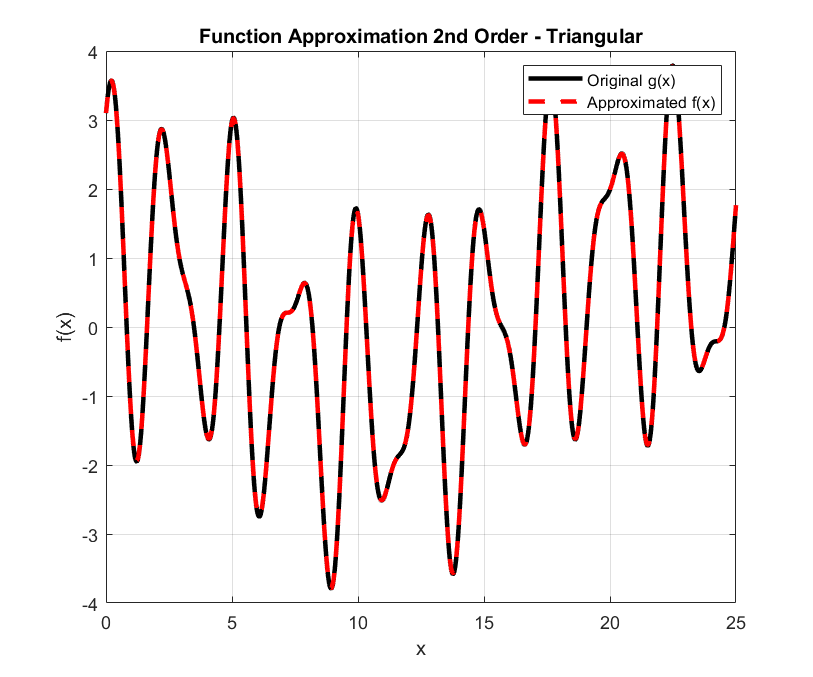
\includegraphics[width=.48\linewidth]{SecondOrder_Triangular_3_2.png}\hfill
  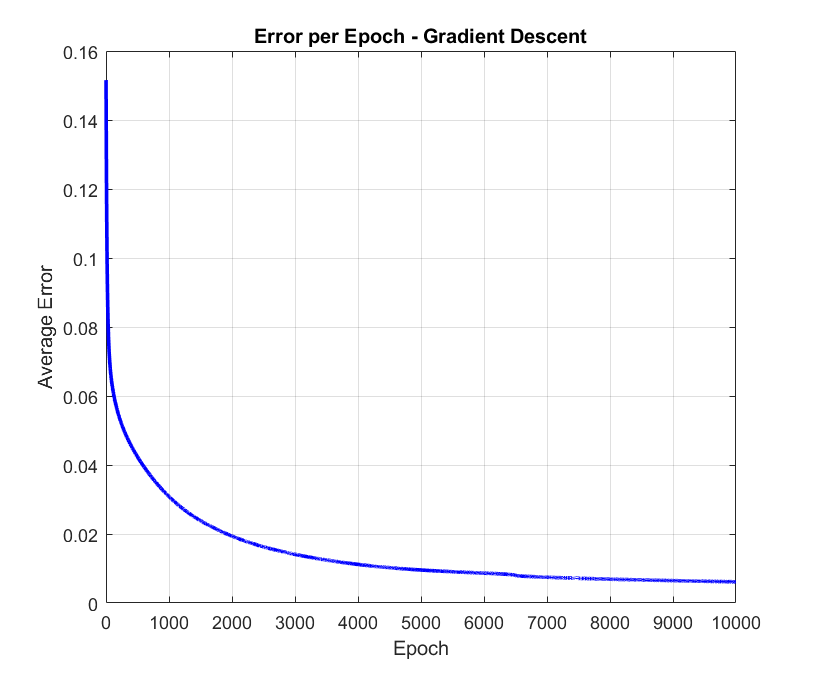
\includegraphics[width=.48\linewidth]{GradientDescent_7_2.png}
  \caption{Second-order triangular design (left) and the training error of the gradient-descent design (right).}
\end{figure}
\end{document}
